\documentclass[11pt]{beamer}
\usetheme{Warsaw}
\usepackage[utf8]{inputenc}
\usepackage[spanish]{babel}
\usepackage{amsmath,amsthm,amssymb} %modos matemáticos y  simbolos
\usepackage{latexsym,amsfonts} %simbolos matematicos
\usepackage{graphicx}
\usepackage{physics} %Simbolos fisicos
\usepackage{array} %mejores formatos de tabla
\usepackage{tabulary}
\usepackage{multirow} %ocupar varias filas en una tabla
\usepackage{fancybox} %recuadros talegas
\usepackage{float} %ubicar graficas
\usepackage{color}
\usepackage{comment}
\usepackage{stackrel}
\usepackage{calligra}
\usepackage{lipsum} % texto de relleno
\usepackage{cite}
\usepackage{pdfpages}
\author{Diego Sarceño}
\title{\href{https://github.com/DSarceno/2022LabSimu201900109/tree/main/SegundoParcial}{Segundo Parcial}}
%\setbeamercovered{transparent} 
%\setbeamertemplate{navigation symbols}{} 
%\logo{} 
%\institute{} 
\date{\today} 
%\subject{\href{Link a Github}{https://github.com/DSarceno/2022LabSimu201900109/tree/main/SegundoParcial}} 
\begin{document}

\begin{frame}
\titlepage
\end{frame}

\AtBeginSection[]
{
    \begin{frame}<beamer>{Contenido}
        \tableofcontents[currentsection]
    \end{frame}
}

\frame{\titlepage}

\frame{
    \frametitle{Contenido}
    \tableofcontents
}


\section{Enunciado del Problema}
\frame{
	\frametitle{Enunciado y Datos del Problema}
	Se elabora un estudio del comportamiento de los precios del combustible tipo regular, asumiendo que
estos tiene un comportamiento lineal y en base a la tabla de datos:
	\begin{itemize}
		\item Una gráfica que compare los valores tabulados y la recta que mejor aproxima el comportamiento.
		\item Asumiendo que el gobierno tiene un tope de 30 quetzales por galón, determine en cuanto tiempo se
llegara a ese tope si el precio mantiene este comportamiento.
	\end{itemize}
}

\frame{
	\frametitle{Enunciado y Datos del Problema}
	\begin{table}[H]
		\centering
		\caption{Datos}
		\begin{tabular}{||c|c||}
			\hline
			\hline
			Semana & Precio (Q/galón) \\
			\hline
			\hline
			$1$ & $20.20$ \\
			$2$ & $20.90$ \\
			$3$ & $20.60$ \\
			$4$ & $21.30$ \\
			$5$ & $20.75$ \\
			$6$ & $22.05$ \\
			$7$ & $23.62$ \\
			$8$ & $22.95$ \\
			$9$ & $23.80$ \\
			$10$ & $24.00$ \\
			\hline
			\hline
		\end{tabular}				
	\end{table}
}


\section{Metodología}
\frame{
	\frametitle{Análisis del Problema}
	Dado el conjunto de datos se realizó un ajuste lineal con dos métodos, utilizando \textit{gnuplot} y el método de mínimos cuadrados. \\
	Para el ajuste usando gnuplot se utilizaron las dos siguientes líneas de código: \\[0.25cm]
	\texttt{\# Función sobre la cual se ajustan los datos} \\
	\texttt{f(x) = a*x + b \# en este caso función lineal} \\
	\texttt{\# Comando fit para el Ajuste} \\
	\texttt{fit f(x) 'data.dat' using 1:2 via a,b}
}

\frame{
	\frametitle{Análisis del Problema}
	Utilizando mínimos cuadrados para encontrar la pendiente y el intercepto se tiene
	$$ m = \frac{n\displaystyle\sum _{k = 0} ^n x_k y_k - \qty(\displaystyle\sum _{k = 0} ^n x_k) \qty(\displaystyle\sum _{k = 0} ^n y_k)}{n\displaystyle\sum _{k = 0} ^n x_k ^2 - \qty(\displaystyle\sum _{k = 0} ^n x_k)^2} $$
	$$ b = \frac{\displaystyle\sum _{k = 0} ^n y_k - m\displaystyle\sum _{k = 0} ^n x_k}{n} $$
}

\section{Solución}

\frame{
	\frametitle{Diagrama de Flujo}
	\begin{figure}[H]
		\centering
		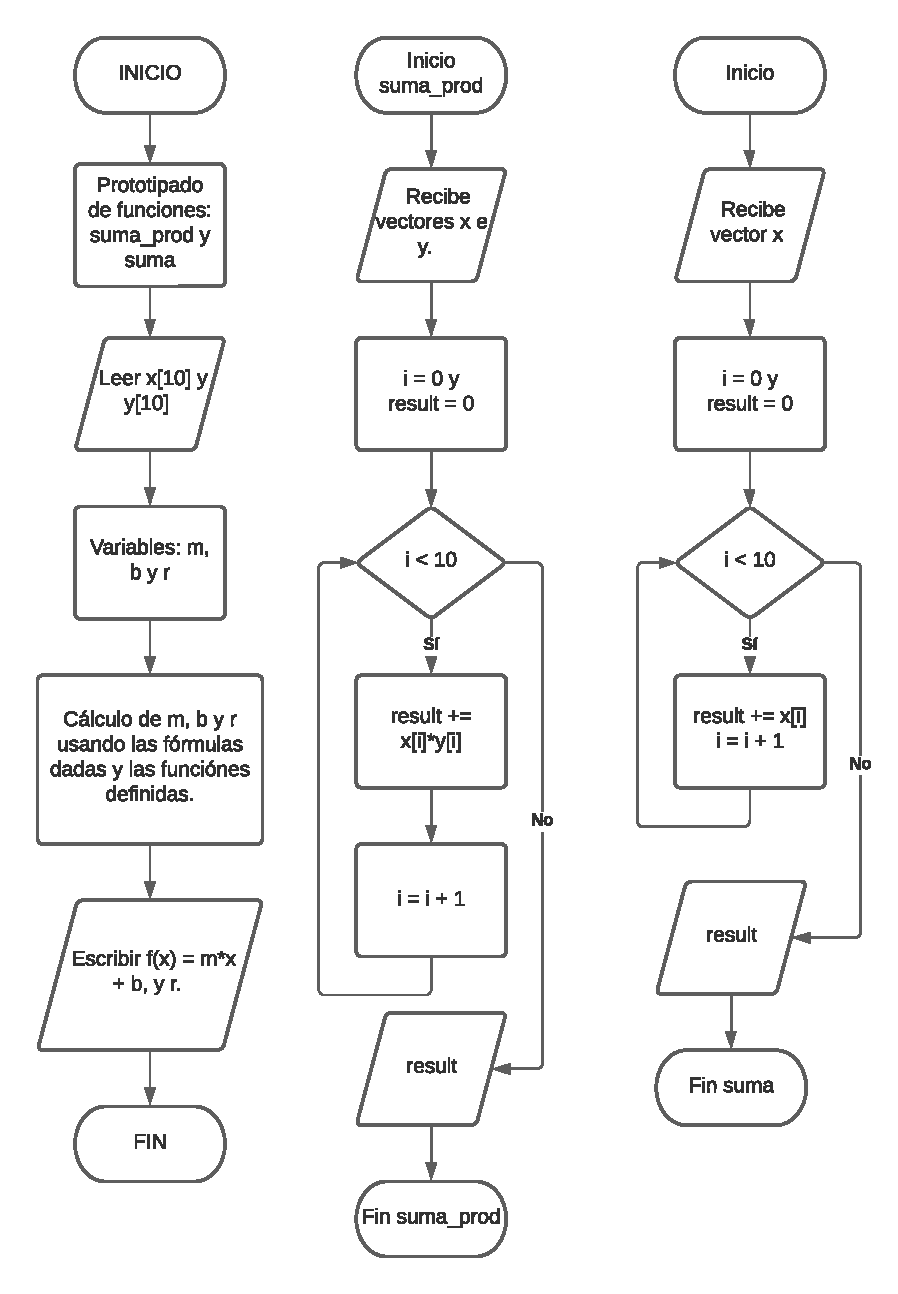
\includegraphics[scale=0.3]{img/problema1.pdf}
		\caption{Diagrama de Flujo Mínimos Cuadrados}
	\end{figure}
}

\frame{
	\frametitle{Variables y Funciones}
	\begin{itemize}
		\item \texttt{x}: Vector que almacena las coordenadas "x" de los datos.
		\item \texttt{y}: Vector que almacena las coordenadas 'y' de los datos.
		\item \texttt{i}: iterador en las funciónes.
		\item \texttt{n}: longitud de los vectores.
		\item \texttt{m}: Pendiente de la recta.
		\item \texttt{b}: Intercepto de la recta.
		\item \texttt{r}: Coeficiente de correlación.
		\item \texttt{suma\_prod(vector,vector)}: función que calcula el producto punto entre ambos vectores.
		\item \texttt{suma(vector)}: Función que calcula la suma de todas las coordenadas del vector.
	\end{itemize}
}

\frame{
	\frametitle{Código Gnuplot}
	\begin{figure}[H]
		\centering
		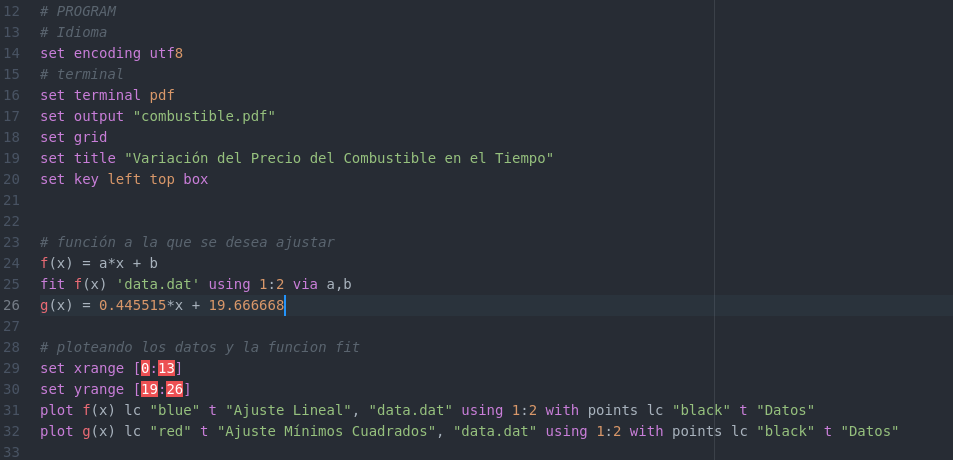
\includegraphics[scale=0.3]{img/codigognuplot.png}
		\caption{Codigo para el ajuste en \textit{gnuplot} y la graficación de los datos y los dos ajustes.}
	\end{figure}
}

\frame{
	\frametitle{Resultados Obtenidos}
	\begin{table}[H]
		\centering
		\caption{Resultados mediante los dos procedimientos dados}
		\begin{tabular}{||c||c|c||}
			\hline
			\hline
				Método & $m$ & $b$ \\
			\hline
			\hline
				Mínimos Cuadrados & $0.445515$ & $19.666668$ \\
			\hline
				Ajuste Gnuplot & $0.445515$ & $19.6667$ \\
			\hline
			\hline
		\end{tabular}
	\end{table}
	El tiempo que le toma al combustible alcanzar su precio límite es de: $23.19$ semanas ($23$ semanas $1$ día y $\approx 8$ horas, para ser más exacto). Esto despejando la ecuación $g(x) = 0.445515x + 19.666668 = 30$ generada con mínimos cuadrados.
}


\frame{
	\frametitle{Gráficas de las Rectas Encontradas}
	\begin{figure}[H]
		\centering
		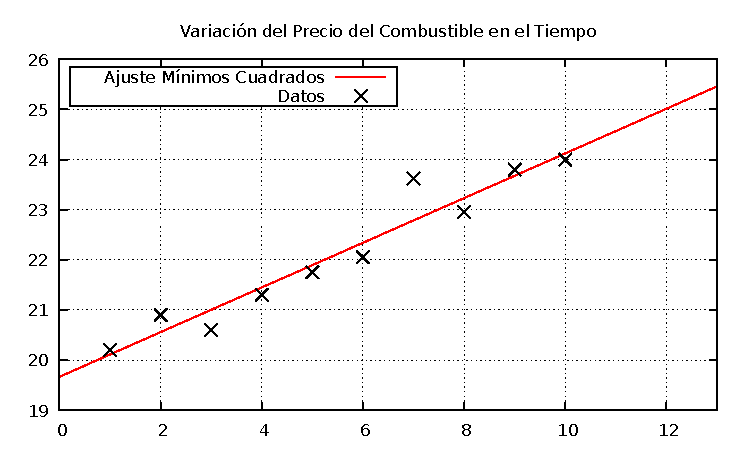
\includegraphics[scale=0.7]{img/c2.pdf}
		\caption{Grafica de recta y datos.}
	\end{figure}
}


\frame{
	\frametitle{Gráficas de las Rectas Encontradas}
	\begin{figure}[H]
		\centering
		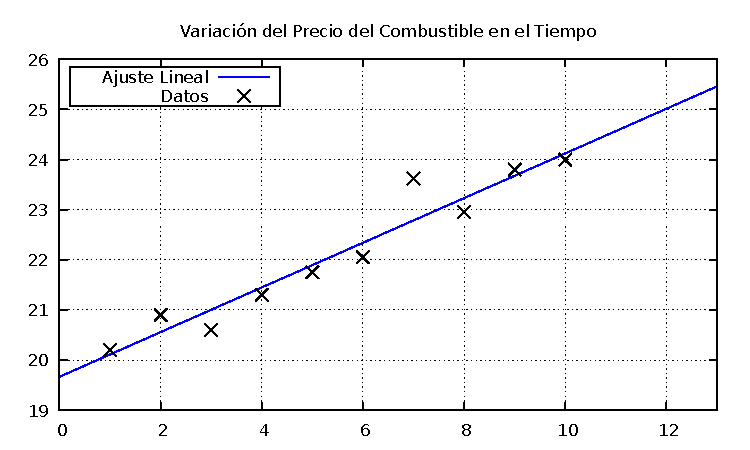
\includegraphics[scale=0.7]{img/c1.pdf}
		\caption{Grafica de recta y datos.}
	\end{figure}
}

\frame{
	\centering
	\vspace{1cm}
	GRACIAS POR SU ATENCIÓN $<3$ \\ (El link a la carpeta de github esta en el título de la presentación.)
}














\end{document}